% Options for packages loaded elsewhere
\PassOptionsToPackage{unicode}{hyperref}
\PassOptionsToPackage{hyphens}{url}
\PassOptionsToPackage{dvipsnames,svgnames,x11names}{xcolor}
%
\documentclass[
  letterpaper,
  DIV=11,
  numbers=noendperiod]{scrartcl}

\usepackage{amsmath,amssymb}
\usepackage{iftex}
\ifPDFTeX
  \usepackage[T1]{fontenc}
  \usepackage[utf8]{inputenc}
  \usepackage{textcomp} % provide euro and other symbols
\else % if luatex or xetex
  \usepackage{unicode-math}
  \defaultfontfeatures{Scale=MatchLowercase}
  \defaultfontfeatures[\rmfamily]{Ligatures=TeX,Scale=1}
\fi
\usepackage{lmodern}
\ifPDFTeX\else  
    % xetex/luatex font selection
\fi
% Use upquote if available, for straight quotes in verbatim environments
\IfFileExists{upquote.sty}{\usepackage{upquote}}{}
\IfFileExists{microtype.sty}{% use microtype if available
  \usepackage[]{microtype}
  \UseMicrotypeSet[protrusion]{basicmath} % disable protrusion for tt fonts
}{}
\makeatletter
\@ifundefined{KOMAClassName}{% if non-KOMA class
  \IfFileExists{parskip.sty}{%
    \usepackage{parskip}
  }{% else
    \setlength{\parindent}{0pt}
    \setlength{\parskip}{6pt plus 2pt minus 1pt}}
}{% if KOMA class
  \KOMAoptions{parskip=half}}
\makeatother
\usepackage{xcolor}
\setlength{\emergencystretch}{3em} % prevent overfull lines
\setcounter{secnumdepth}{5}
% Make \paragraph and \subparagraph free-standing
\makeatletter
\ifx\paragraph\undefined\else
  \let\oldparagraph\paragraph
  \renewcommand{\paragraph}{
    \@ifstar
      \xxxParagraphStar
      \xxxParagraphNoStar
  }
  \newcommand{\xxxParagraphStar}[1]{\oldparagraph*{#1}\mbox{}}
  \newcommand{\xxxParagraphNoStar}[1]{\oldparagraph{#1}\mbox{}}
\fi
\ifx\subparagraph\undefined\else
  \let\oldsubparagraph\subparagraph
  \renewcommand{\subparagraph}{
    \@ifstar
      \xxxSubParagraphStar
      \xxxSubParagraphNoStar
  }
  \newcommand{\xxxSubParagraphStar}[1]{\oldsubparagraph*{#1}\mbox{}}
  \newcommand{\xxxSubParagraphNoStar}[1]{\oldsubparagraph{#1}\mbox{}}
\fi
\makeatother


\providecommand{\tightlist}{%
  \setlength{\itemsep}{0pt}\setlength{\parskip}{0pt}}\usepackage{longtable,booktabs,array}
\usepackage{calc} % for calculating minipage widths
% Correct order of tables after \paragraph or \subparagraph
\usepackage{etoolbox}
\makeatletter
\patchcmd\longtable{\par}{\if@noskipsec\mbox{}\fi\par}{}{}
\makeatother
% Allow footnotes in longtable head/foot
\IfFileExists{footnotehyper.sty}{\usepackage{footnotehyper}}{\usepackage{footnote}}
\makesavenoteenv{longtable}
\usepackage{graphicx}
\makeatletter
\def\maxwidth{\ifdim\Gin@nat@width>\linewidth\linewidth\else\Gin@nat@width\fi}
\def\maxheight{\ifdim\Gin@nat@height>\textheight\textheight\else\Gin@nat@height\fi}
\makeatother
% Scale images if necessary, so that they will not overflow the page
% margins by default, and it is still possible to overwrite the defaults
% using explicit options in \includegraphics[width, height, ...]{}
\setkeys{Gin}{width=\maxwidth,height=\maxheight,keepaspectratio}
% Set default figure placement to htbp
\makeatletter
\def\fps@figure{htbp}
\makeatother
% definitions for citeproc citations
\NewDocumentCommand\citeproctext{}{}
\NewDocumentCommand\citeproc{mm}{%
  \begingroup\def\citeproctext{#2}\cite{#1}\endgroup}
\makeatletter
 % allow citations to break across lines
 \let\@cite@ofmt\@firstofone
 % avoid brackets around text for \cite:
 \def\@biblabel#1{}
 \def\@cite#1#2{{#1\if@tempswa , #2\fi}}
\makeatother
\newlength{\cslhangindent}
\setlength{\cslhangindent}{1.5em}
\newlength{\csllabelwidth}
\setlength{\csllabelwidth}{3em}
\newenvironment{CSLReferences}[2] % #1 hanging-indent, #2 entry-spacing
 {\begin{list}{}{%
  \setlength{\itemindent}{0pt}
  \setlength{\leftmargin}{0pt}
  \setlength{\parsep}{0pt}
  % turn on hanging indent if param 1 is 1
  \ifodd #1
   \setlength{\leftmargin}{\cslhangindent}
   \setlength{\itemindent}{-1\cslhangindent}
  \fi
  % set entry spacing
  \setlength{\itemsep}{#2\baselineskip}}}
 {\end{list}}
\usepackage{calc}
\newcommand{\CSLBlock}[1]{\hfill\break\parbox[t]{\linewidth}{\strut\ignorespaces#1\strut}}
\newcommand{\CSLLeftMargin}[1]{\parbox[t]{\csllabelwidth}{\strut#1\strut}}
\newcommand{\CSLRightInline}[1]{\parbox[t]{\linewidth - \csllabelwidth}{\strut#1\strut}}
\newcommand{\CSLIndent}[1]{\hspace{\cslhangindent}#1}

\usepackage{booktabs}
\usepackage{longtable}
\usepackage{array}
\usepackage{multirow}
\usepackage{wrapfig}
\usepackage{float}
\usepackage{colortbl}
\usepackage{pdflscape}
\usepackage{tabu}
\usepackage{threeparttable}
\usepackage{threeparttablex}
\usepackage[normalem]{ulem}
\usepackage{makecell}
\usepackage{xcolor}
\KOMAoption{captions}{tableheading}
\makeatletter
\@ifpackageloaded{caption}{}{\usepackage{caption}}
\AtBeginDocument{%
\ifdefined\contentsname
  \renewcommand*\contentsname{Table of contents}
\else
  \newcommand\contentsname{Table of contents}
\fi
\ifdefined\listfigurename
  \renewcommand*\listfigurename{List of Figures}
\else
  \newcommand\listfigurename{List of Figures}
\fi
\ifdefined\listtablename
  \renewcommand*\listtablename{List of Tables}
\else
  \newcommand\listtablename{List of Tables}
\fi
\ifdefined\figurename
  \renewcommand*\figurename{Figure}
\else
  \newcommand\figurename{Figure}
\fi
\ifdefined\tablename
  \renewcommand*\tablename{Table}
\else
  \newcommand\tablename{Table}
\fi
}
\@ifpackageloaded{float}{}{\usepackage{float}}
\floatstyle{ruled}
\@ifundefined{c@chapter}{\newfloat{codelisting}{h}{lop}}{\newfloat{codelisting}{h}{lop}[chapter]}
\floatname{codelisting}{Listing}
\newcommand*\listoflistings{\listof{codelisting}{List of Listings}}
\makeatother
\makeatletter
\makeatother
\makeatletter
\@ifpackageloaded{caption}{}{\usepackage{caption}}
\@ifpackageloaded{subcaption}{}{\usepackage{subcaption}}
\makeatother

\ifLuaTeX
  \usepackage{selnolig}  % disable illegal ligatures
\fi
\usepackage{bookmark}

\IfFileExists{xurl.sty}{\usepackage{xurl}}{} % add URL line breaks if available
\urlstyle{same} % disable monospaced font for URLs
\hypersetup{
  pdftitle={Global Life Expectancy: Unraveling Health and Economic Determinants (2015-2020)},
  pdfauthor={Yanfei Huang},
  colorlinks=true,
  linkcolor={blue},
  filecolor={Maroon},
  citecolor={Blue},
  urlcolor={Blue},
  pdfcreator={LaTeX via pandoc}}


\title{Global Life Expectancy: Unraveling Health and Economic
Determinants (2015-2020)\thanks{Code and data are available at:
\url{https://github.com/wendyhuan/lifeexpectancy}.}}
\usepackage{etoolbox}
\makeatletter
\providecommand{\subtitle}[1]{% add subtitle to \maketitle
  \apptocmd{\@title}{\par {\large #1 \par}}{}{}
}
\makeatother
\subtitle{Multiple Linear Regression Analyzing Critical Factors Shaping
Life Expectancy}
\author{Yanfei Huang}
\date{December 2, 2024}

\begin{document}
\maketitle
\begin{abstract}
This paper analyze life expectancy and its determinants through 184
countries and make the prediction of people from different Income Group.
Multiple Linear regression is used to deploying the life expectanc with
gender, income and region. Predictions of life expectancy of people from
different income group is made according to these essential predictors.
The finding indicates that the life expectancy is tend to get higher as
the economic class grows. And we predict that the average age of person
from low, lower-middle, upper-middle and high are 65,70, 75,80. The
result of this paper will help in suggesting a country which area should
be given importance in order to efficiently improve the life expectancy
of its population.
\end{abstract}

\renewcommand*\contentsname{Table of contents}
{
\hypersetup{linkcolor=}
\setcounter{tocdepth}{3}
\tableofcontents
}

\section{Introduction}\label{introduction}

Life expectancy is a critical measure of a population's overall health
and well-being, shaped by various factors such as gender, geographic
location and economic group. The index of life expectancy is generally
served as a benchmark for income group, indicating the effectiveness of
interventions in reducing mortality and improving well-being. Higher
life expectancy is believed to linked to stronger physical factor,
better living standards, and geographic location. Conversely, low life
expectancy often signals systemic challenges such as weaker health,
lower economic situation, and inadequate healthcare access of different
region. (\textbf{socialdeterminantsofhealth?}).

The primary goal of this paper is to determine which factors play a
statistically significant role in driving lower life expectancy values
and to offer actionable insights based on different income group.
According to the World Bank Income Group, the countries are classified
into low, lower-middle, upper-middle, and high based on the country's
Gross National Income. Using Multiple Linear Regression model and
Bayesian model, this study focuses on understanding the relationship
between Gender, Region and different income group in predicting life
expectancy across different countries. By identifying and analyzing
these predictors, the study aims to highlight actionable aspects for
policymakers to target in their efforts to improve population longevity
effectively.

Related Research has shown that there exist difference between men and
women related with biological, behavioral, and socioeconomic factors,
highlighting that gender-specific health behaviors and societal roles
influence longevity (\textbf{GenderandLifeExpectancy?}). Higher-income
individuals tend to live longer due to better access to healthcare and
healthier lifestyles, with notable regional disparities even within
similar income groups (\textbf{IncomeGroupsandLongevity?}).
Additionally, regional socioeconomic differences on health outcomes,
especially life expectancy. It emphasizes that addressing regional
inequities in wealth and resources is essential for improving population
health globally. (\textbf{RegionalVariations?}).

Findings from this paper reveal that countries of higher income group
tend to achieve higher life expectancy, while factors like lower income
and poverty region emerge as significant obstacles. The analysis
underscores the importance of targeted interventions in key areas such
as healthcare accessibility and economic equity to address disparities
in life expectancy. This study further contributes to a deeper
understanding of how predictive modeling under different country status
can inform public health strategies and policy-making on a global scale.

The ultimate goal is to assist policymakers in developing evidence-based
strategies that can enhance population health outcomes. The approach of
this paper not only emphasizes the importance of equitable access to
healthcare but also contributes to a broader understanding of the
multifaceted factors shaping life expectancy globally. By highlighting
the interplay between various determinants, this study contributes to a
broader understanding of the challenges and opportunities in improving
life expectancy on a global scale.

The structure of the paper is as follows: Section~\ref{sec-data}
outlines the data sources and variables considered, followed by the
model setup in Section~\ref{sec-modset} and justification in
\textbf{?@sec-modjust}. The results in \textbf{?@sec-result} presents
the key findings of the analysis, with a discussion on the implications.
\textbf{?@sec-discussion} then discusses potential limitations and
suggestions for future research. \textbf{?@sec-appx} provides additional
detailed information about the data, model and methodology.

\section{Data}\label{sec-data}

\subsection{Overview}\label{overview}

The data used in this analysis originates from The World Health
Organization's (WHO) and Global Health Observatory (GHO)
(\textbf{lifeexpectancy?}). This data-set related to life expectancy,
health factors for 184 countries has been collected from WHO data
repository website and its corresponding economic data was collected
from United Nation website. Among all categories of health-related
factors only those socio-economic factors on the national level were
chosen for global scale analysis.

This analysis uses the statistical programming language R (R Core Team
2023) and several libraries, including \texttt{tidyverse}
(\textbf{tidyverse?}), \texttt{janitor} (\textbf{janitor?}),
\texttt{knitr} (\textbf{knitr?}), \texttt{dplyr} (\textbf{dplyr?}),
\texttt{arrow} (\textbf{arrow?}), \texttt{purrr} (\textbf{purrr?}),
\texttt{sf} (\textbf{sf?}), and \texttt{here} (\textbf{here?}) for data
manipulation. \texttt{ggplot2} (\textbf{ggplot?}), \texttt{ggcorrplot}
(\textbf{ggcorrplot?}) and \texttt{kableExtra} (\textbf{kableExtra?})
for visualization. The dataset covers various predictors conducted
across multiple countries, capturing the support for a country to
determine the predicting factor which is contributing to lower value of
life expectancy.

\subsection{Measurement}\label{measurement}

The measurement process refers to how real-world factors---such as the
Gender, geographic location of a country and income group - are
translated into numerical entries representing life expectancy in a
dataset. Each entry captures the average life expectancy of individuals
in a specific country during a given year.

\textbf{Life Expectancy (\texttt{Life\ Expectancy})}: This variable,
life expectancy at birth, represents the number of years a person is
expected to live , assuming current mortality conditions persist. It is
derived using data from national health records, the World Health
Organization (WHO) and Global Health Observatory (GHO). The data on the
raw dataset is recorded as a range of age. For simple analysis, we drop
the range and take the average of year with one decimal. The values are
calculated and represented in age between 10.1 to 87.4.

\textbf{Income Group(\texttt{Income\_Group})}: This is a categorical
variable that classifies countries into four groups by the country's
Gross National Income according to the latest index from World Bank
Income Group. The countries are classified into low, lower-middle,
upper-middle, and high under the standard as follow. Low-income
economies is defined as a country with a gross national income less than
\$1135, lower-middle is between the range to \$1136 to \$4465,
upper-middle in the range of \$4465 to \$13845 and high is more than
\$13846.

\textbf{Gender(\texttt{Gender})}: The gender of the population of each
country is included as a categorical variable (Male/Female/Both Sex).

\textbf{Region(Region)}: This is a categorical variable that classifies
the geographic location of the countries. It is mapped one by one by the
name of the country. The data is stored as the name of the
continent(`Africa', `Oceania', `Asia', `Europe', `North America', `South
America').

\subsection{Data Cleaning}\label{data-cleaning}

The raw life expectancy data underwent a several cleaning steps to
ensure it was accurate, consistent and ready for analysis. The goal of
this cleaning process is to create a table including income group (high,
upper middle, lower middle, low), gender (Male, Female, Both Sex),
region (Asia, Europe, North America, South America, Africa, Oceania) as
rows and life expectancy as column.

To make such table, we first select and rename key variables from raw
data to focus on relevant information. To make the subsequent analysis
easier, we then convert variables to the proper data types and eliminate
the rows that have missing data values. To keep things neat, we organize
the decimal for every piece of numerical data and drop the percentage
symbol. The income group column and the region column was not given in
the raw dataset. We created a mapping over country name to four income
group according to the index given by World Bank Income Group and save
the data under ``Income\_Group''. We as well made a mapping to the
countries according to its continent and saved as ``Region''. We again
merge the table, removing repeated columns and rows. For easier
visualization, we created four tables, which are grouped by life
expectancy at age 60, life expectancy at birth, life expectancy at birth
of Male and life expectancy at birth of Female.

The cleaned dataset was then saved as both CSV and Parquet file for
efficient storage and further analysis.

More information on the data cleaning process can be found in
\textbf{?@sec-appx}.

\subsection{Outcome Variables}\label{outcome-variables}

The outcome variable is \textbf{\texttt{Life\ Expendency}}. This is the
primary dependent variable that the model is designed to predict. It
represents the average number of years a person is expected to live,
under the condition that current mortality conditions persist. The model
seeks to identify the variables affecting this average.

To examine the differences in life expectancy under the same variables,
we separate the data into developed and developing countries, where
developed country are generally believed to have higher life expectancy.
Figure~\ref{fig-expectancy} displays density of the historical data of
life expectancy across 195 countries from 2000 to 2015, comparing
developing to developed countries.The average age of most developed
country is approximately 80, while the majority developing countries
typically have average life expectancy around mid-seventies.

\begin{figure}

\centering{

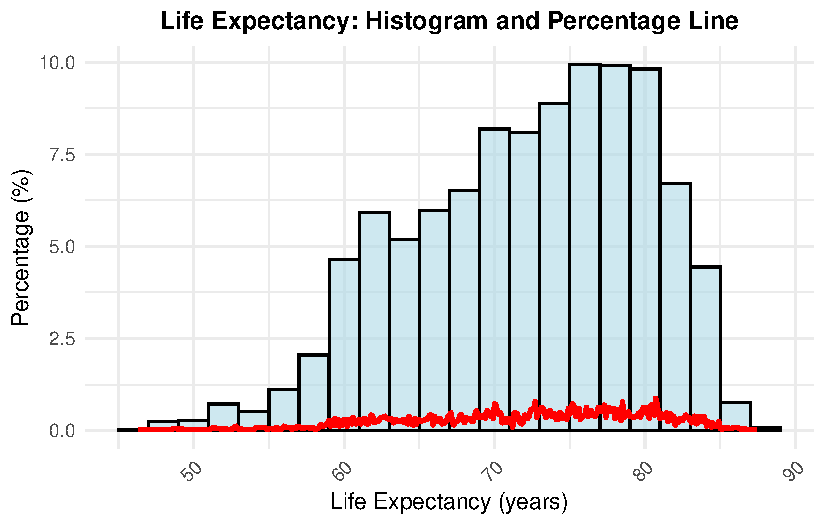
\includegraphics{paper_files/figure-pdf/fig-expectancy-1.pdf}

}

\caption{\label{fig-expectancy}This histogram shows the distribution of
the percentage of life expectancy.}

\end{figure}%

\subsection{Predictor Variables}\label{predictor-variables}

The \textbf{predictor variables} (or independent variables) are the
factors believed to influence the life expectancy:

\begin{enumerate}
\def\labelenumi{\arabic{enumi}.}
\tightlist
\item
  \textbf{Income Group(\texttt{Income\_Group})}: The income group of a
  country is the key factor influencing the life expectancy. This
  variable provides context for comparing life expectancy between
  different levels of country income group. The division of the life
  expectancy by the income group of a country because income levels
  often correlate strongly with various factors affecting health and
  longevity. Higher income countries typically have more resources to
  invest in robust healthcare systems, with better living conditions
  while lower income countries often face challenges such as inadequate
  healthcare infrastructure and malnutrition.
\end{enumerate}

Following by the four income group, we would like to see the
distribution of the income group of 184 WHO member countries.
(\textbf{fid-income?}) shows that there are 55 countries at the high
income group, 26 countries at low income group, 54 countries at the
lower-middle group while there are 49 countries at the upper-middle
group. With significant less low income countries, we expect to see the
life expectancy lie in a comparably higher range. On the other hand,
there might exist sever outliers dropping the mean.

\begin{enumerate}
\def\labelenumi{\arabic{enumi}.}
\setcounter{enumi}{1}
\item
  \textbf{Gender(\texttt{Gender})}: The gender of the population of each
  country is included as a categorical variable (Male/Female/Both Sex).
  This is a key variable in the dataset because gender has been fully
  recognized connected with the biological physical factor which
  directly effect the life expectancy. Figure~\ref{fig-gender} shows
  that the with an stable average of 74, life expectancy of female is
  constantly higher than male's average of 70. The line plot reveals a
  steady increase until 2019, followed by a sharp decline in 2020, which
  is assumed to be associated with the impact of COVID-19.
\item
  \textbf{Region(Region)}: This is a categorical variable that
  classifies the geographic location of the countries. It is mapped one
  by one by the name of the country. The data is stored as the name of
  the continent(`Africa', `Oceania', `Asia', `Europe', `North America',
  `South America'). Figure~\ref{fig-region} indicates that with the
  number of 54, Africa has the most WHO member countries. Both Asia and
  Europe has 43 countries,listing in the middle while the other three
  continent has the significant less number of countries. North America
  has 22 countries, South America has 12 countries and Oceania has the
  least, 10 countries.
\end{enumerate}

\begin{figure}

\centering{

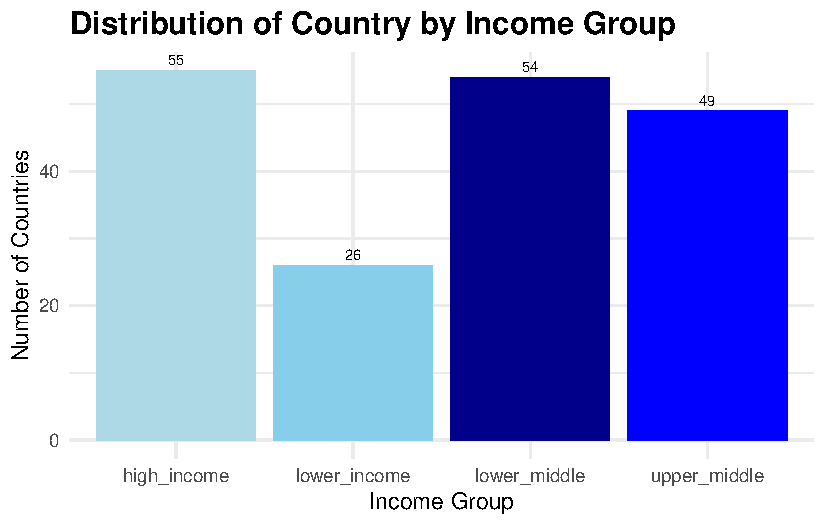
\includegraphics{paper_files/figure-pdf/fig-income-1.pdf}

}

\caption{\label{fig-income}Distribution of country income group.}

\end{figure}%

\begin{figure}

\centering{

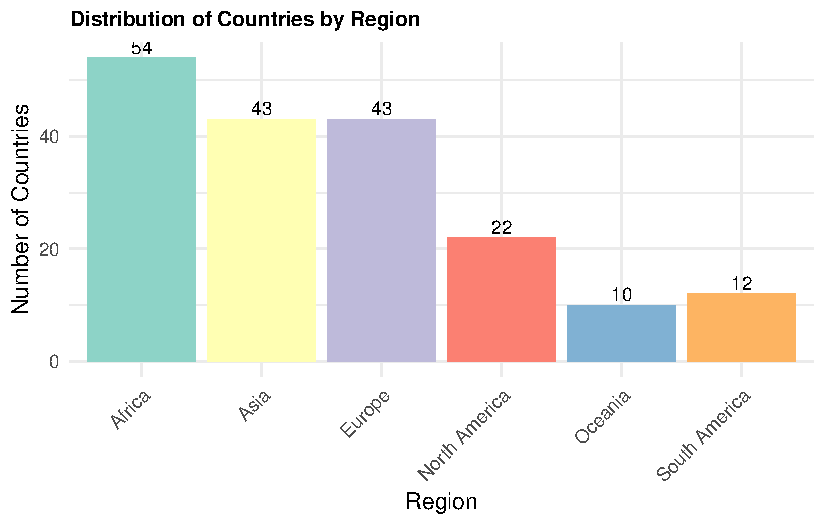
\includegraphics{paper_files/figure-pdf/fig-region-1.pdf}

}

\caption{\label{fig-region}Distribution of different region of the 184
countries. Africa has the most countries with an number of 54. Asia and
Europe has the same amount of 43, North America has 22 countries while
the other two continent has almost the same amount of countries.}

\end{figure}%

\begin{figure}

\centering{

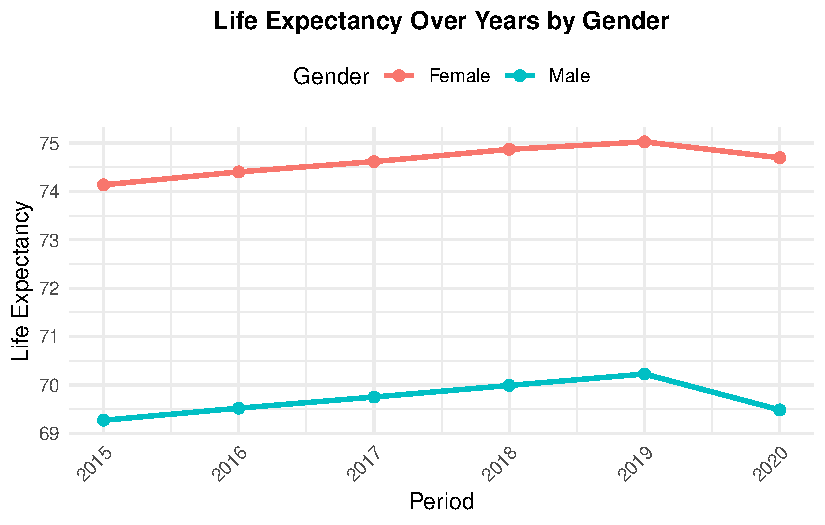
\includegraphics{paper_files/figure-pdf/fig-gender-1.pdf}

}

\caption{\label{fig-gender}Distribution of gender each year. The average
of female life expectancy is approximately 74 around years, constantly
higher than male's average of 70. Compared to male, female's life
expectancy is marginally more steady.}

\end{figure}%

\subsection{Basic Data Summary}\label{basic-data-summary}

The table below shows the basic summary of the mean, median, max,
standard deviation, variance and sample size of life expectancy. We
could tell that the average of the life expectancy from the 6 years is
45.9, with a large standard deviation of 26.9. The max of the life
expectancy is 87.4, among all 6624 rows of data. The standard deviation
and variance are extremely high because of the range of data is large,
in other words, because the mean and median are 45.9 and 37.7, compared
to the max 87.4, there is likely some outliers in the data creating such
a high standard deviation and variance.

\begin{figure}

\centering{

\begin{table}
\centering
\caption{Summary Statistics of Life Expectancy}
\centering
\begin{tabular}[t]{c|c|c|c|c|c}
\hline
Mean & Median & Max & Standard Deviation & Variance & N\\
\hline
45.9 & 37.7 & 87.4 & 26.9 & 724.2 & 6624\\
\hline
\end{tabular}
\end{table}

}

\caption{\label{fig-summary}Summary statistics of the number of life
expectancy over countries and years.}

\end{figure}%

\section{Model}\label{model}

\subsection{Model set-up}\label{sec-modset}

The goal of the Bayesian model is to incorporate prior knowledge, such
as insights from previous studies or analyses, into the selection of the
model. To predict the outcome of the life expectancy of people from
different regions, in this paper, we developed a linear regression
models using R (R Core Team 2023). The outcome variable,
\textbf{\texttt{Life\ Expectancy}}, is a continuous and represents the
average number of years a person is expected to live, assuming all
related resources remain constant throughout their lifetime. The model
aim to estimate and predict the life expectancy of people under
different gender, region and income group. The normal Gaussian
distribution is effective when used for modeling scenarios where the
residuals of the data aare assumed to be independent nd normally
distributed around the regression line. The GAM allows for capturing
potential non-linear relationships between the predictors and the
outcome.

The model is specified as follows:

\begin{align} 
y_i|\mu_i, \sigma &\sim \mbox{Normal}(\mu_i, \sigma) \\
\mu_i &= \alpha + \beta_i + \gamma_i\\
\alpha &\sim \mbox{Normal}(0, 2.5) \\
\beta &\sim \mbox{Normal}(0, 2.5) \\
\gamma &\sim \mbox{Normal}(0, 2.5) \\
\sigma &\sim \mbox{Exponential}(1)
\end{align}

Where:

\begin{itemize}
\item
  \(yi\) is the outcome variable (Life Expectancy)for the i-th country.
\item
  \(_i\) represents the expected value of \(yi\), modeled as a linear
  combination of the predictors: Gender, Region, and Income Group.
\item
  \(Gender\) is the gender of the individual.
\item
  \(Income Group\) is the income group of the country.
\item
  \(\epsilon_i\) is the error term, assumed to be normally distributed
  with a mean of 0 and constant variance \(ϵ_i​∼N(0,\sigma^2)\)
\end{itemize}

This GAM model allows for smooth, non-linear effects of continuous
predictors (\textbf{\texttt{age}} and \textbf{\texttt{races\_count}})
while keeping the categorical predictors
(\textbf{\texttt{Income\_Group}} and \textbf{\texttt{iaaf\_category}})
in a linear framework.

Appendix~\ref{sec-model-details}.

We run the model in R (R Core Team 2023) using the \texttt{rstanarm}
package of Goodrich et al. (2022). We use the default priors from
\texttt{rstanarm}.

\subsubsection{Model justification}\label{model-justification}

We expect a positive relationship between the size of the wings and time
spent aloft. In particular\ldots{}

We can use maths by including latex between dollar signs, for instance
\(\theta\).

\paragraph{Model Validation}\label{model-validation}

RMSE

Out-of- Sample testing

\section{Results}\label{results}

Our results are summarized in Table~\ref{tbl-modelresults}.

\begin{enumerate}
\def\labelenumi{\arabic{enumi}.}
\tightlist
\item
  check different continent has its different life expectancy.
\item
  compare the develop country with
\item
  check the shcooling year of develop countries to developing country,
  showing a relationship between shcooling with the life expenctancy.
\item
\end{enumerate}

\section{Discussion}\label{discussion}

\subsection{First discussion point}\label{sec-first-point}

If my paper were 10 pages, then should be be at least 2.5 pages. The
discussion is a chance to show off what you know and what you learnt
from all this.

\subsection{Second discussion point}\label{second-discussion-point}

Please don't use these as sub-heading labels - change them to be what
your point actually is.

\subsection{Life Expectancy at 60}\label{life-expectancy-at-60}

The life expectancy at 60 means that how long is a person expected to
live at 60 instead of at birth.

\subsection{Weaknesses and next steps}\label{weaknesses-and-next-steps}

Weaknesses and next steps should also be included.

\newpage

\appendix

\section{Appendix}\label{sec-appendix}

\subsection{Data Cleaning Notes}\label{data-cleaning-notes}

We began by importing the raw dataset using the read\_csv function from
the tidyverse package. To focus our analysis on more relevant variables,
we selected specific columns, such as percentage of expenditure of the
country, total health expenditure by government .etc., omitting any
unnecessary columns.

We filter out the rows containing NA values in any of the selected
columns for reducing the noise and simpler further analysis..

We then renaming columns for clarity. For example, we changed
`Income.composition.of.resources' into `IncomeComposition' , making it
easier for anyone working with the data to read and understand what each
variable represents.

Each column is rounded using the round function, specifying the desired
number of decimal places for each. Columns not mentioned in mutate
remain unchanged. This ensures a flexible and precise cleaning process
tailored to further compairation and graphing.

We also modified the country name of `Republic of Korea' under Country
variable to `South Korea' to avoid misunderstanding of North Korea.

We also created a new variable called Continent, which indicates which
continent does the country comes from in order to provide a geographical
context to the analysis. Life expectancy may be higher in developed
regions like Europe or North America compared to regions like
Sub-Saharan Africa due to differences in healthcare, living standards,
and economic development.

We also wrapped the cleaning process in a tryCatch block in order to
mitigate any errors that arose throughout the cleaning process.

After completing the cleaning, we saved the final dataset in both
Parquet and CSV formats for later analysis.

\subsection{Data Cleaning Table}\label{data-cleaning-table}

\subsubsection{Idealized Survey}\label{idealized-survey}

\textbf{Survey: Understanding Life Expectancy and Influencing Factor}

Thank you for participating in this survey. This survey aims to gather
insights into the factors influencing life expectancy, including health
expenditure, education, ethnicity, government spending on healthcare,
and income levels. Your responses will help us understand individual
perspectives and experiences towards national policy. Participation is
voluntary, and your answers will remain anonymous.

\textbf{Contact Information:} If you have any questions about the survey
or the data collection process, please contact

\textbf{Survey Coordinator}: Yanfei Huang\\
\textbf{Email}: yanfei.huang@mail.utoronto.ca

\textbf{Section 1: Personal Health Expenditure}

\textbf{1.What percentage of your monthly income do you spend on
healthcare (e.g., insurance, medications, doctor visits)?}

\begin{itemize}
\tightlist
\item
  Less than 5\%
\item
  5\%--10\%
\item
  10\%--20\%
\item
  More than 20\%
\end{itemize}

\textbf{2.Do you or your household have health insurance coverage?}

\begin{itemize}
\tightlist
\item
  Yes
\item
  No
\end{itemize}

\textbf{3. How frequently do you visit a healthcare
professional(eg.doctors, nurse) in a year?}

\begin{itemize}
\tightlist
\item
  0-1 times
\item
  2-5 times
\item
  6-10 times
\item
  More than 10 times
\end{itemize}

\textbf{Section 2: Education Background}

\textbf{4.What is the highest level of education you have completed?}

\begin{itemize}
\tightlist
\item
  No formal education
\item
  Primary school
\item
  Secondary school
\item
  College or university degree
\item
  Postgraduate degree
\end{itemize}

\textbf{5.How many years of formal schooling have you completed?}

Please write the number: \_\_\_\_\_\_\_

\textbf{Section 3: Ethnicity and Geographic Factors}

\textbf{6.Which of the following best describes your ethnicity?}

\begin{itemize}
\tightlist
\item
  African
\item
  Asian
\item
  European
\item
  Hispanic or Latino
\item
  Middle Eastern
\item
  Indigenous
\item
  Other (please specify): \_\_\_\_\_\_\_
\end{itemize}

\textbf{7.What's the distance to the nearest healthcare facility from
your residence?}

\begin{itemize}
\tightlist
\item
  Less than 1 km
\item
  1-5 km
\item
  More than 5 km
\end{itemize}

\textbf{Section 4: Government Expenditure on Healthcare}

\textbf{8.Are health services in your country subsidized by the
govenment?}

\begin{itemize}
\tightlist
\item
  Yes, fully subsidized
\item
  Yes, partially subsidized
\item
  No
\end{itemize}

\textbf{9. What is the approximate cost of your most recent healthcare
visit (in local currency)?}

Please write the amount \_\_\_\_\_\_\_

\textbf{10.Do public healthcare facilities in your area provide all the
services you need?}

\begin{itemize}
\tightlist
\item
  Yes
\item
  No
\item
  Not applicable
\end{itemize}

\textbf{Section 5: Income and Development Factor}

\textbf{11.What is your approximate monthly household income after
taxes?(in local currency)}

\begin{itemize}
\tightlist
\item
  Less than 1,000
\item
  1,000 - 2,999
\item
  3,000 - 4,999
\item
  5,000 - 7,999
\item
  8,000 - 10,999
\item
  More than 11,000
\item
  Prefer not to say
\end{itemize}

\textbf{12.How would you describe your current financial situation?}

\begin{itemize}
\tightlist
\item
  Struggling to make ends meet
\item
  Just getting by
\item
  Comfortable, but not wealthy
\item
  Financially secure
\item
  Wealthy
\item
  Prefer not to say
\end{itemize}

\textbf{13.How often do you have difficulty affording basic healthcare
(medical visits, medications, etc.)?}

\begin{itemize}
\tightlist
\item
  Never
\item
  Rarely
\item
  Sometimes
\item
  Often
\item
  Always
\item
  Prefer not to say
\end{itemize}

\textbf{Final Section}

Thank you for completing this survey! Your responses will help capture
information about economic conditions, access to healthcare and
education, and basic living standards, which are critical for
understanding life expectancy predictors and the impact of socioeconomic
factors on health outcomes.

\section{Additional data details}\label{additional-data-details}

\section{Model details}\label{sec-model-details}

\subsection{Additional graph for
analysis}\label{additional-graph-for-analysis}

\subsection{Posterior predictive
check}\label{posterior-predictive-check}

In \textbf{?@fig-ppcheckandposteriorvsprior-1} we implement a posterior
predictive check. This shows\ldots{}

In \textbf{?@fig-ppcheckandposteriorvsprior-2} we compare the posterior
with the prior. This shows\ldots{}

\begin{figure}

\begin{minipage}{0.50\linewidth}
Examining how the model fits, and is affected by, the
data\end{minipage}%

\end{figure}%

\subsection{Diagnostics}\label{diagnostics}

\textbf{?@fig-stanareyouokay-1} is a trace plot. It shows\ldots{} This
suggests\ldots{}

\textbf{?@fig-stanareyouokay-2} is a Rhat plot. It shows\ldots{} This
suggests\ldots{}

\begin{figure}

\begin{minipage}{0.50\linewidth}
Checking the convergence of the MCMC algorithm\end{minipage}%

\end{figure}%

\newpage

\section*{References}\label{references}
\addcontentsline{toc}{section}{References}

\phantomsection\label{refs}
\begin{CSLReferences}{1}{0}
\bibitem[\citeproctext]{ref-rstanarm}
Goodrich, Ben, Jonah Gabry, Imad Ali, and Sam Brilleman. 2022.
{``{rstanarm: {Bayesian} applied regression modeling via {Stan}}.''}
\url{https://mc-stan.org/rstanarm/}.

\bibitem[\citeproctext]{ref-citeR}
R Core Team. 2023. \emph{{R: A Language and Environment for Statistical
Computing}}. Vienna, Austria: R Foundation for Statistical Computing.
\url{https://www.R-project.org/}.

\end{CSLReferences}




\end{document}
